\documentclass{beamer}


\usepackage{tikz}
\usetikzlibrary{positioning,calc}
\usetikzlibrary{shapes.geometric}
\usetikzlibrary{backgrounds}% only to show the bounding box
\usetikzlibrary{shapes,arrows}
\usepackage{pgfplots}
\usepackage{pgfplotstable}
\usetikzlibrary{pgfplots.groupplots}
\pgfplotsset{compat=1.12}
\usepackage{appendixnumberbeamer}
\usepackage{amsmath}
\date{8th June 2016}
\usetheme{firedrake}

\title{Thetis}
\subtitle{a three dimensional baroclinic ocean model}
\author[Tuomas K\"{a}rn\"{a}]{
Tuomas K\"{a}rn\"{a}\inst{1} \and
Ant\'{o}nio Baptista\inst{1} \and
Stephan Kramer\inst{2} \and
\underline{Lawrence Mitchell}\inst{2} \and
David Ham\inst{2}
}


\institute[CMOP]{
\inst{1}
Oregon Health \& Science University\\
\inst{2}
Imperial College London
}


\date{13th July 2016}

\renewcommand{\vec}[1]{\ensuremath{\boldsymbol{#1}}}
\newcommand{\ddt}[1]{\frac{\partial #1}{\partial t}}
\newcommand{\dd}[2]{\frac{\partial #1}{\partial #2}}
\newcommand{\zhat}{\hat{\vec{z}}}
\newcommand{\W}{\ensuremath{\mathbb{W}}}
\newcommand{\nablah}{\ensuremath{\vec{\nabla}_{\!\!h}}}

\DeclareMathOperator{\grad}{grad}
\let\div\relax
\DeclareMathOperator{\div}{div}
\DeclareMathOperator{\curl}{curl}
\newcommand{\inner}[2]{\ensuremath{\langle #1, #2 \rangle}}
\graphicspath{{./\jobname.figures/}}

\newcommand{\arxivlink}[2]{%
  \href{http://www.arxiv.org/abs/#1}%
  {{\small\texttt{arXiv:\,#1\,[#2]}}}%
}
\newcommand{\doilink}[1]{%
  \href{http://dx.doi.org/#1}%
  {{\small\texttt{doi:\,#1}{}}}%
}
\usepackage[url=false,
            doi=true,
            isbn=false,
            style=authoryear,
            firstinits=true,
            uniquename=init,
            backend=biber]{biblatex}

\setbeamertemplate{bibliography item}{}
\renewcommand{\bibfont}{\footnotesize}
\addbibresource{references.bib}

\setlength{\bibitemsep}{1ex}

\renewbibmacro{in:}{}
\DeclareFieldFormat[article]{volume}{\textbf{#1}}
\DeclareFieldFormat{doi}{%
  doi\addcolon%
  {\scriptsize\ifhyperref{\href{http://dx.doi.org/#1}{\nolinkurl{#1}}}
    {\nolinkurl{#1}}}}
\AtEveryBibitem{%
\clearfield{pages}%
\clearfield{issue}%
\clearfield{number}%
}

\usepackage{minted}

\begin{document}

\titlegraphic{\hspace*{-2em}
\includegraphics[height=1.1cm]{cmop-logo}\hfill%
  
\includegraphics[height=1.1cm]{firedrake-word}}

\bgroup
\setbeamertemplate{background}{}
\begin{frame}[standout]
  Firetran!\\
  \arxivlink{1407.2905}{cs.SE}
  \vspace*{1em}\\
  \visible<2>{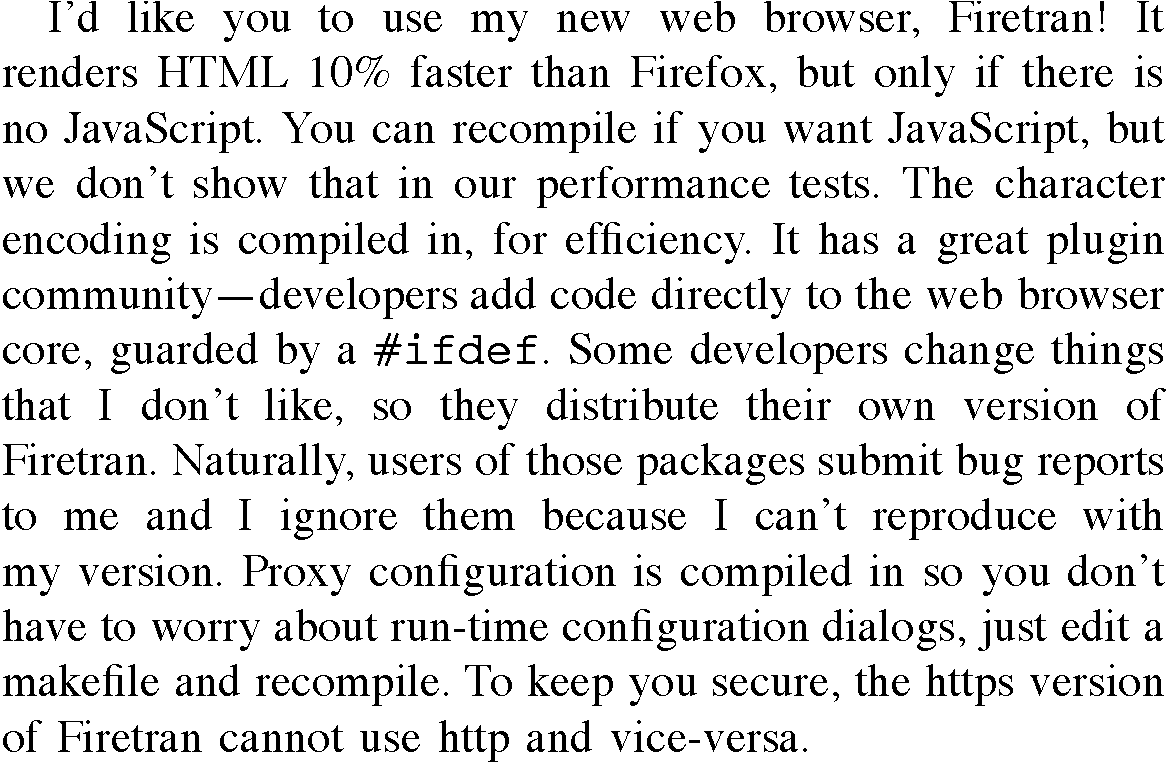
\includegraphics[width=0.75\textwidth]{firetran}}
\end{frame}
\egroup

\maketitle

\section{Motivation}


\begin{frame}[t]
  \frametitle{Why do we need a new coastal ocean model?}
  \begin{itemize}
  \item Structured grids good for global and regional models.
  \item Coastal applications require unstructured grids, which tend to be
    \emph{computationally expensive} and \emph{diffusive}.
  \end{itemize}
  \begin{columns}[t]
    \begin{column}{0.32\textwidth}
      \textbf{Global}
      \begin{center}
        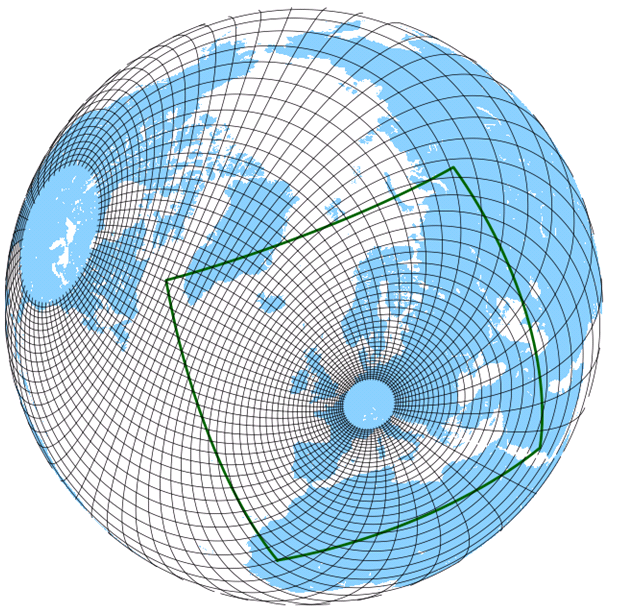
\includegraphics[width=0.95\textwidth]{global-grid}
      \end{center}
    \end{column}
    \begin{column}{0.32\textwidth}
      \textbf{Regional}
      \begin{center}
        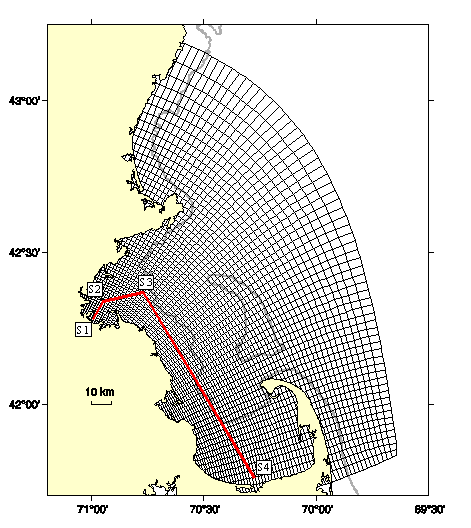
\includegraphics[width=0.95\textwidth]{cape-cod}
      \end{center}
    \end{column}
    \begin{column}{0.32\textwidth}
      \textbf{Coastal/estuary}
      \begin{center}
        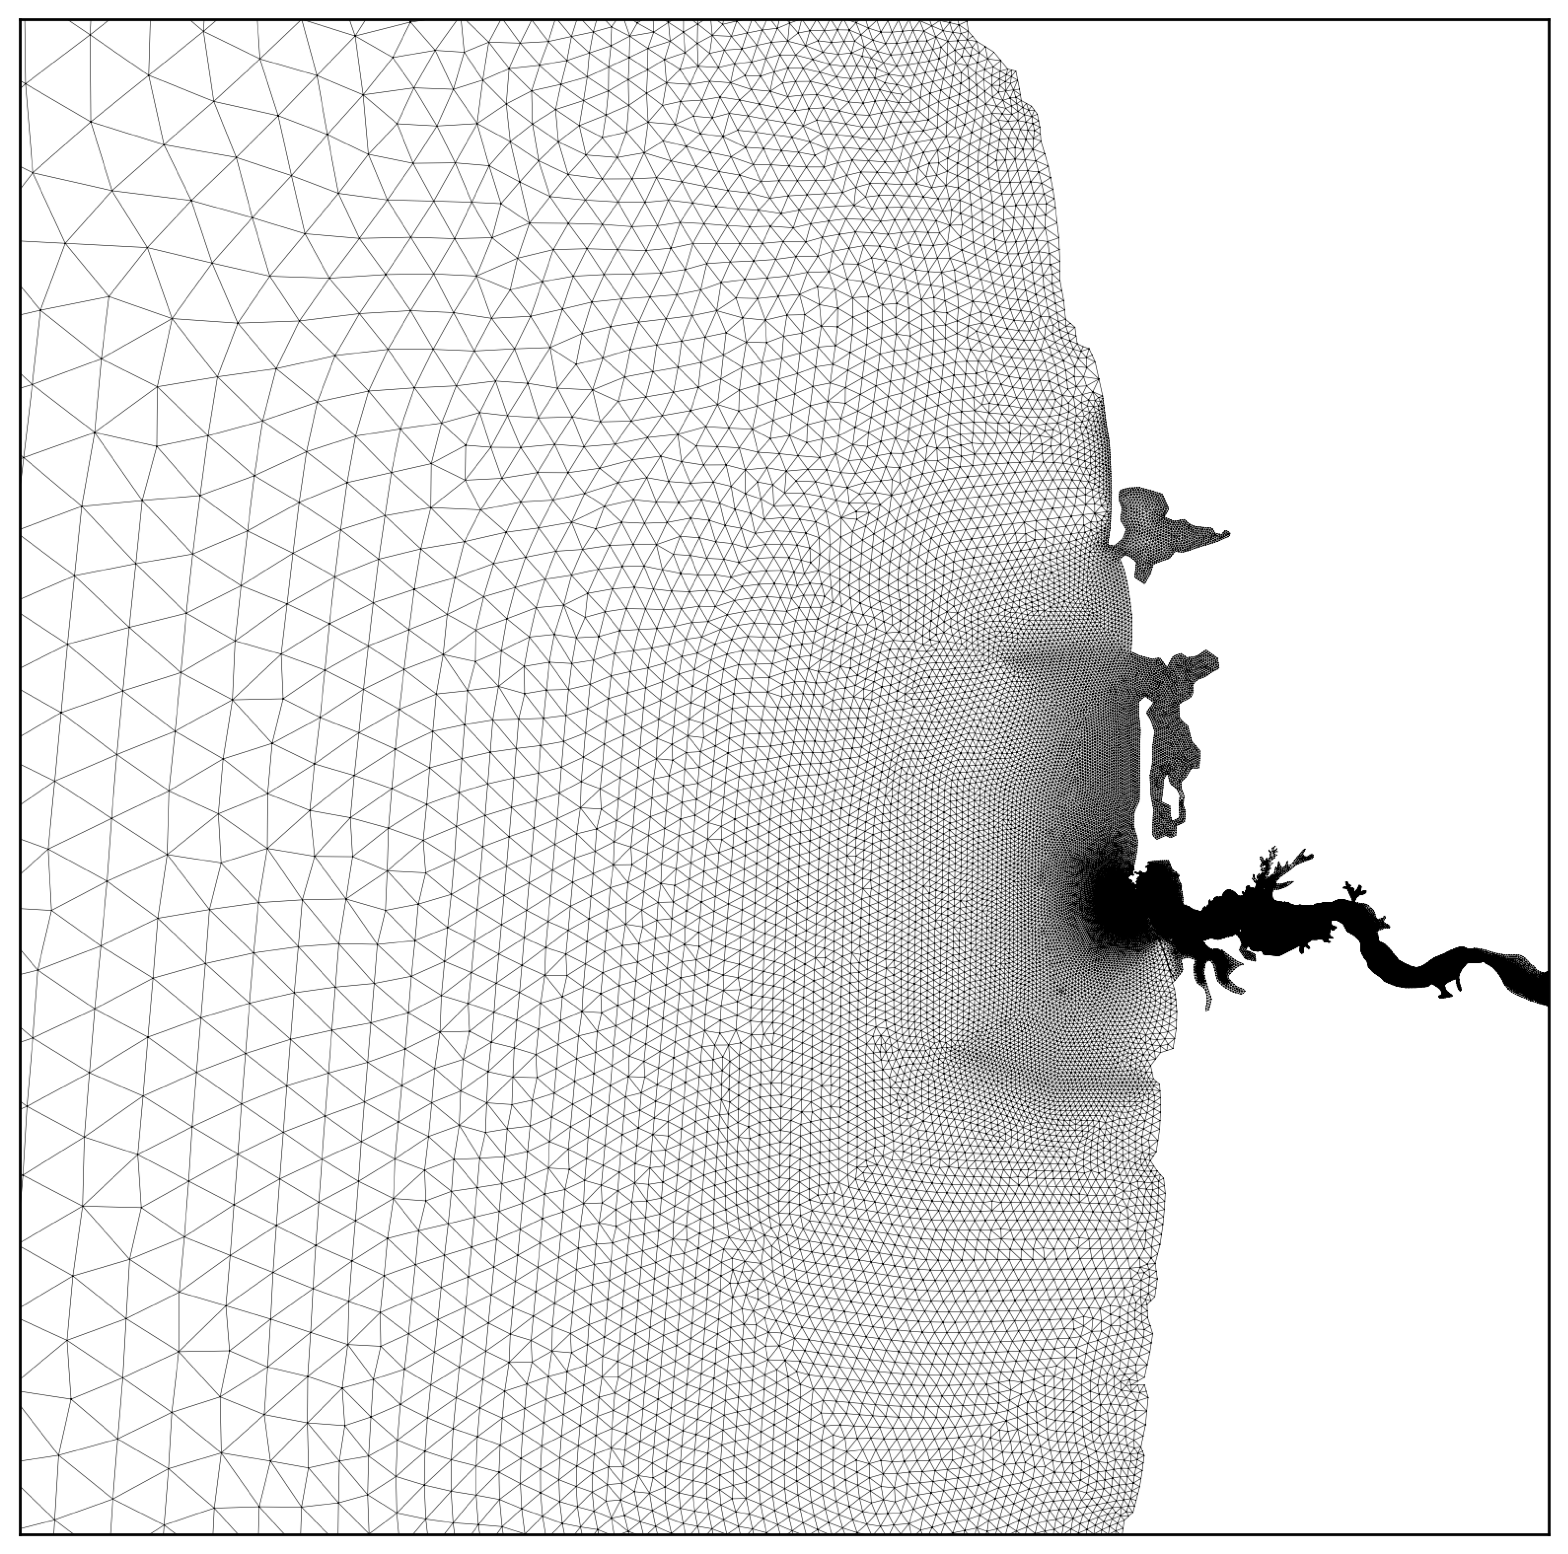
\includegraphics[width=\textwidth]{columbia-river}
      \end{center}
    \end{column}
  \end{columns}
\end{frame}


\begin{frame}[t]
  \frametitle{Columbia River estuary application}
  \begin{columns}[t]
  \begin{column}{0.5\textwidth}
    \begin{itemize}
    \item Complex topography
    \item Energetic tides
    \item Strong river discharge
    \item Strong density gradients
    \item Baroclinic effects very important
    \end{itemize}
    Current model at CMOP (SELFE) is too diffusive \parencite{Karna:2015}.
  \end{column}
  \hspace*{-2em}
  \begin{column}{0.6\textwidth}
    \begin{center}
      \vspace{-2em}
      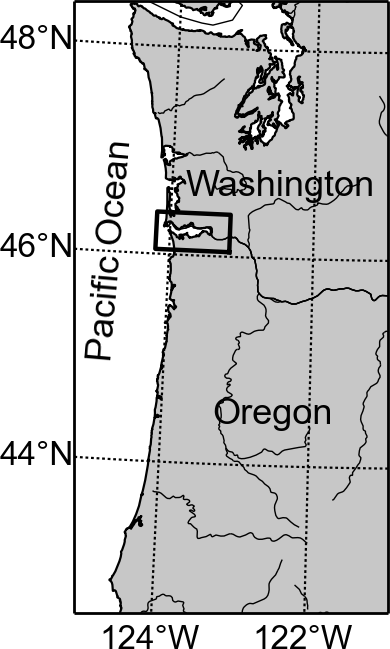
\includegraphics[width=0.3\textwidth]{columbia-river-map}
      \vspace{1em}
      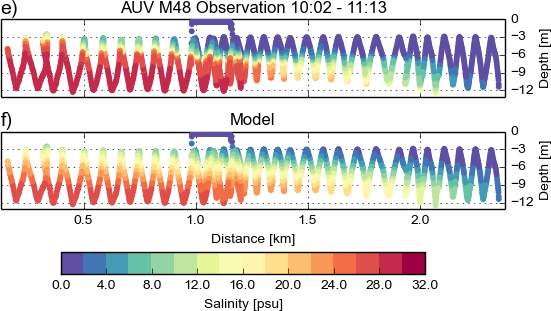
\includegraphics[width=0.75\textwidth]{selfe-salinity}
    \end{center}
  \end{column}
\end{columns}
\end{frame}

\begin{frame}
  \frametitle{Tidal turbine placement}
  \begin{itemize}
  \item Placement of turbines in an array can significantly change
    power generated
  \item Previous optimisations results using 2D shallow-water +
    dolfin-adjoint
  \item Want to move to 3D model
  \item Existing AMCG code (Fluidity) faaar too slow for optimisation
    runs.
  \end{itemize}
\end{frame}
\section{A new model}

\begin{frame}
\frametitle{A new coastal ocean model}
\begin{columns}
  \begin{column}{0.25\textwidth}
    
\includegraphics[width=\textwidth]{thetis_logo}
  \end{column}
  \begin{column}{0.75\textwidth} {\small
      \url{github.com/thetisproject/thetis}}
  \end{column}
\end{columns}
\begin{columns}
  \begin{column}{0.9\textwidth}
    \begin{itemize}
    \item Solves 3D Navier-Stokes equations
    \item Hydrostatic and Boussinesq approximations
    \item Also 2D shallow water model
    \item Implemented using Firedrake
    \end{itemize}
  \end{column}
\end{columns}
\end{frame}

\begin{frame}[allowframebreaks]
\frametitle{Governing equations}
\begin{block}{Horizontal momentum equation, \vec{u}}
  \begin{align*}
    \ddt{\vec{u}} + \nablah \cdot (\vec{u}\vec{u})
    + \dd{(w\vec{u})}{z} +& \\
    f\vec{e}_z\times\vec{u} + g\nablah \eta + g\nablah r &= \nablah
      \cdot (\nu_h \nablah \vec{u}) + \dd{}{z}\left( \nu
        \dd{\vec{u}}{z}\right),
  \end{align*}
\end{block}
\begin{block}{Continuity equation, $w$ (diagnostic)}
  \begin{align*}
    \nablah \cdot \vec{u} + \dd{w}{z} = 0.
  \end{align*}
\end{block}
\pagebreak
Mode split 2D/3D dynamics

\begin{block}{Depth averaged shallow water equations, $\eta$,
    $\bar{\vec{u}}$}
\begin{align*}
\ddt{\eta} + \nablah \cdot ((\eta + h) \bar{\vec{u}}) &= 0, \\
 \ddt{\bar{\vec{u}}} + \bar{\vec{u}} \cdot \nablah\bar{\vec{u}} + f\vec{e}_z\times \bar{\vec{u}}
+ g \nablah \eta + g \frac{1}{H}\int_{-h}^\eta \nablah r \mathsf{d}z &=  \bar{\vec{A}}_H.
\end{align*}
\end{block}
\pagebreak

\begin{block}{Tracers, salinity ($S$) and temperature ($T$)}
\begin{align*}
\ddt{T} + \nablah \cdot (\vec{u} T) + \dd{(wT)}{z} =
 \nablah \cdot (\mu_h \nablah T) + \dd{}{z}\left( \mu  \dd{T}{z}\right).
\end{align*}
\end{block}
\begin{block}{Internal pressure gradient, $\nabla_h r$ (diagnostic)}
  \begin{align*}
    \nablah r &= \frac{1}{\rho_0} \nablah  \int_{z}^\eta  \rho' \mathsf{d}\zeta
  \end{align*}
  with $\rho' = \rho'(T, S)$ the (diagnostic) equation of state.
\end{block}
\pagebreak

\begin{block}{Generic length scale turbulence closure, $\nu$, $\mu$}
  \begin{align*}
    \ddt{k} + \nablah \cdot (\vec{u} k) + \dd{(w k)}{z} &= \dd{}{z}\left(\frac{\nu}{\sigma_k} \dd{k}{z}\right) + P + B - \varepsilon\\
    \dd{\Psi}{t} + \nablah \cdot (\vec{u} \Psi) + \dd{(w k)}{z} &= \dd{}{z}\left(\frac{\nu}{\sigma_\Psi} \dd{\Psi}{z}\right) + \frac{\Psi}{k}(c_1 P + c_3 B - c_2 \varepsilon) \\
    \nu &= c_\nu \sqrt{k} L, \\
    \mu &= c_{\mu} \sqrt{k} L, \\
    L &= \left(c_\mu^0\right)^{-p/n} k^{-m/n} \Psi^{1/n}.
  \end{align*}
  Following \cite{Umlauf:2003}.
\end{block}
\end{frame}

\begin{frame}
  \frametitle{Discretisation}
  3D cells, triangular prisms.
  \begin{block}{DG}
    \begin{itemize}
    \item 2D velocity-pressure pair: $(P_1dg)^2-P_1dg$
    \item 3D velocity in $(P_1dg)^3$, tracers $P_1dg$ otherwise as 2D
    \item Turbulent quantities in $P_0$.
    \end{itemize}
  \end{block}
  \begin{block}{Mimetic pair}
    Support for Gung-Ho-like $H(\div)-L^2$ mimetic discretisation.
    Currently $RT_1-P_1dg$.
  \end{block}
\end{frame}


\begin{frame}[t]
  \frametitle{Time integration}
  \begin{block}{Implicit terms}
    \begin{itemize}
    \item Surface gravity waves: $\Theta$ scheme.
    \item Vertical diffusion: backward Euler
    \end{itemize}
  \end{block}
  \begin{block}{Explicit terms}
    \begin{itemize}
    \item SSPRK(3,3), third order, three stage SSP, CFL coefficient of 1.
    \item ERK-LPUM2, second order, three stage SSP, CFL coefficient of
      2.  \cite{Higueras:2014}.
    \end{itemize}
  \end{block}
  \begin{block}{Tracer advection}
    SSPRK scheme + Kuzmin slope limiters (positivity preserving)
  \end{block}
\end{frame}

\begin{frame}[t]
\frametitle{Time integration}
\begin{itemize}
\item Most restrictive CFL conditions
  \begin{itemize}
  \item Free surface waves: {\scriptsize $\Delta t < \Delta x / \sqrt{gH}$}
  \item Vertical diffusion: {\scriptsize $\Delta t < \Delta z^2 / \nu$}
  \item Horizontal advection: {\scriptsize $\Delta t < \Delta x / U$}
  \end{itemize}
\item<2-> 2D shallow water equations
  \begin{itemize}
  \item Free surface waves are treated with $\Theta$ scheme
  \item Rest of the terms are explicit
  \end{itemize}
\item<3-> 3D momentum and tracer equations
  \begin{itemize}
  \item Vertical diffusion is treated implicitly
  \item Rest of the terms are explicit
  \end{itemize}
\item<4-> Horizontal advection treated explicitly
\end{itemize}
\visible<5->{Easy to switch treatment of individual terms from explicit to implicit.}
\end{frame}

\begin{frame}
  \frametitle{Why Firedrake?}
  \begin{block}{Requirements}
    \begin{itemize}
    \item[\checkmark] Extruded meshes
    \item[\checkmark] Non-affine (prismatic) cells must be treated properly
    \item[\checkmark] Need to treat horizontal and vertical dynamics separately
    \item[\checkmark] Programmability
    \item[\checkmark] Good computational performance
    \item[\checkmark] Access to non-variational aspects in code generation (slope
      limiters, ...)
    \end{itemize}
  \end{block}
\end{frame}

\section{Some test cases}

\begin{frame}
  \frametitle{Idealized river plume test: Thetis is less diffusive}
  \begin{columns}
    \begin{column}{0.75\textwidth}
        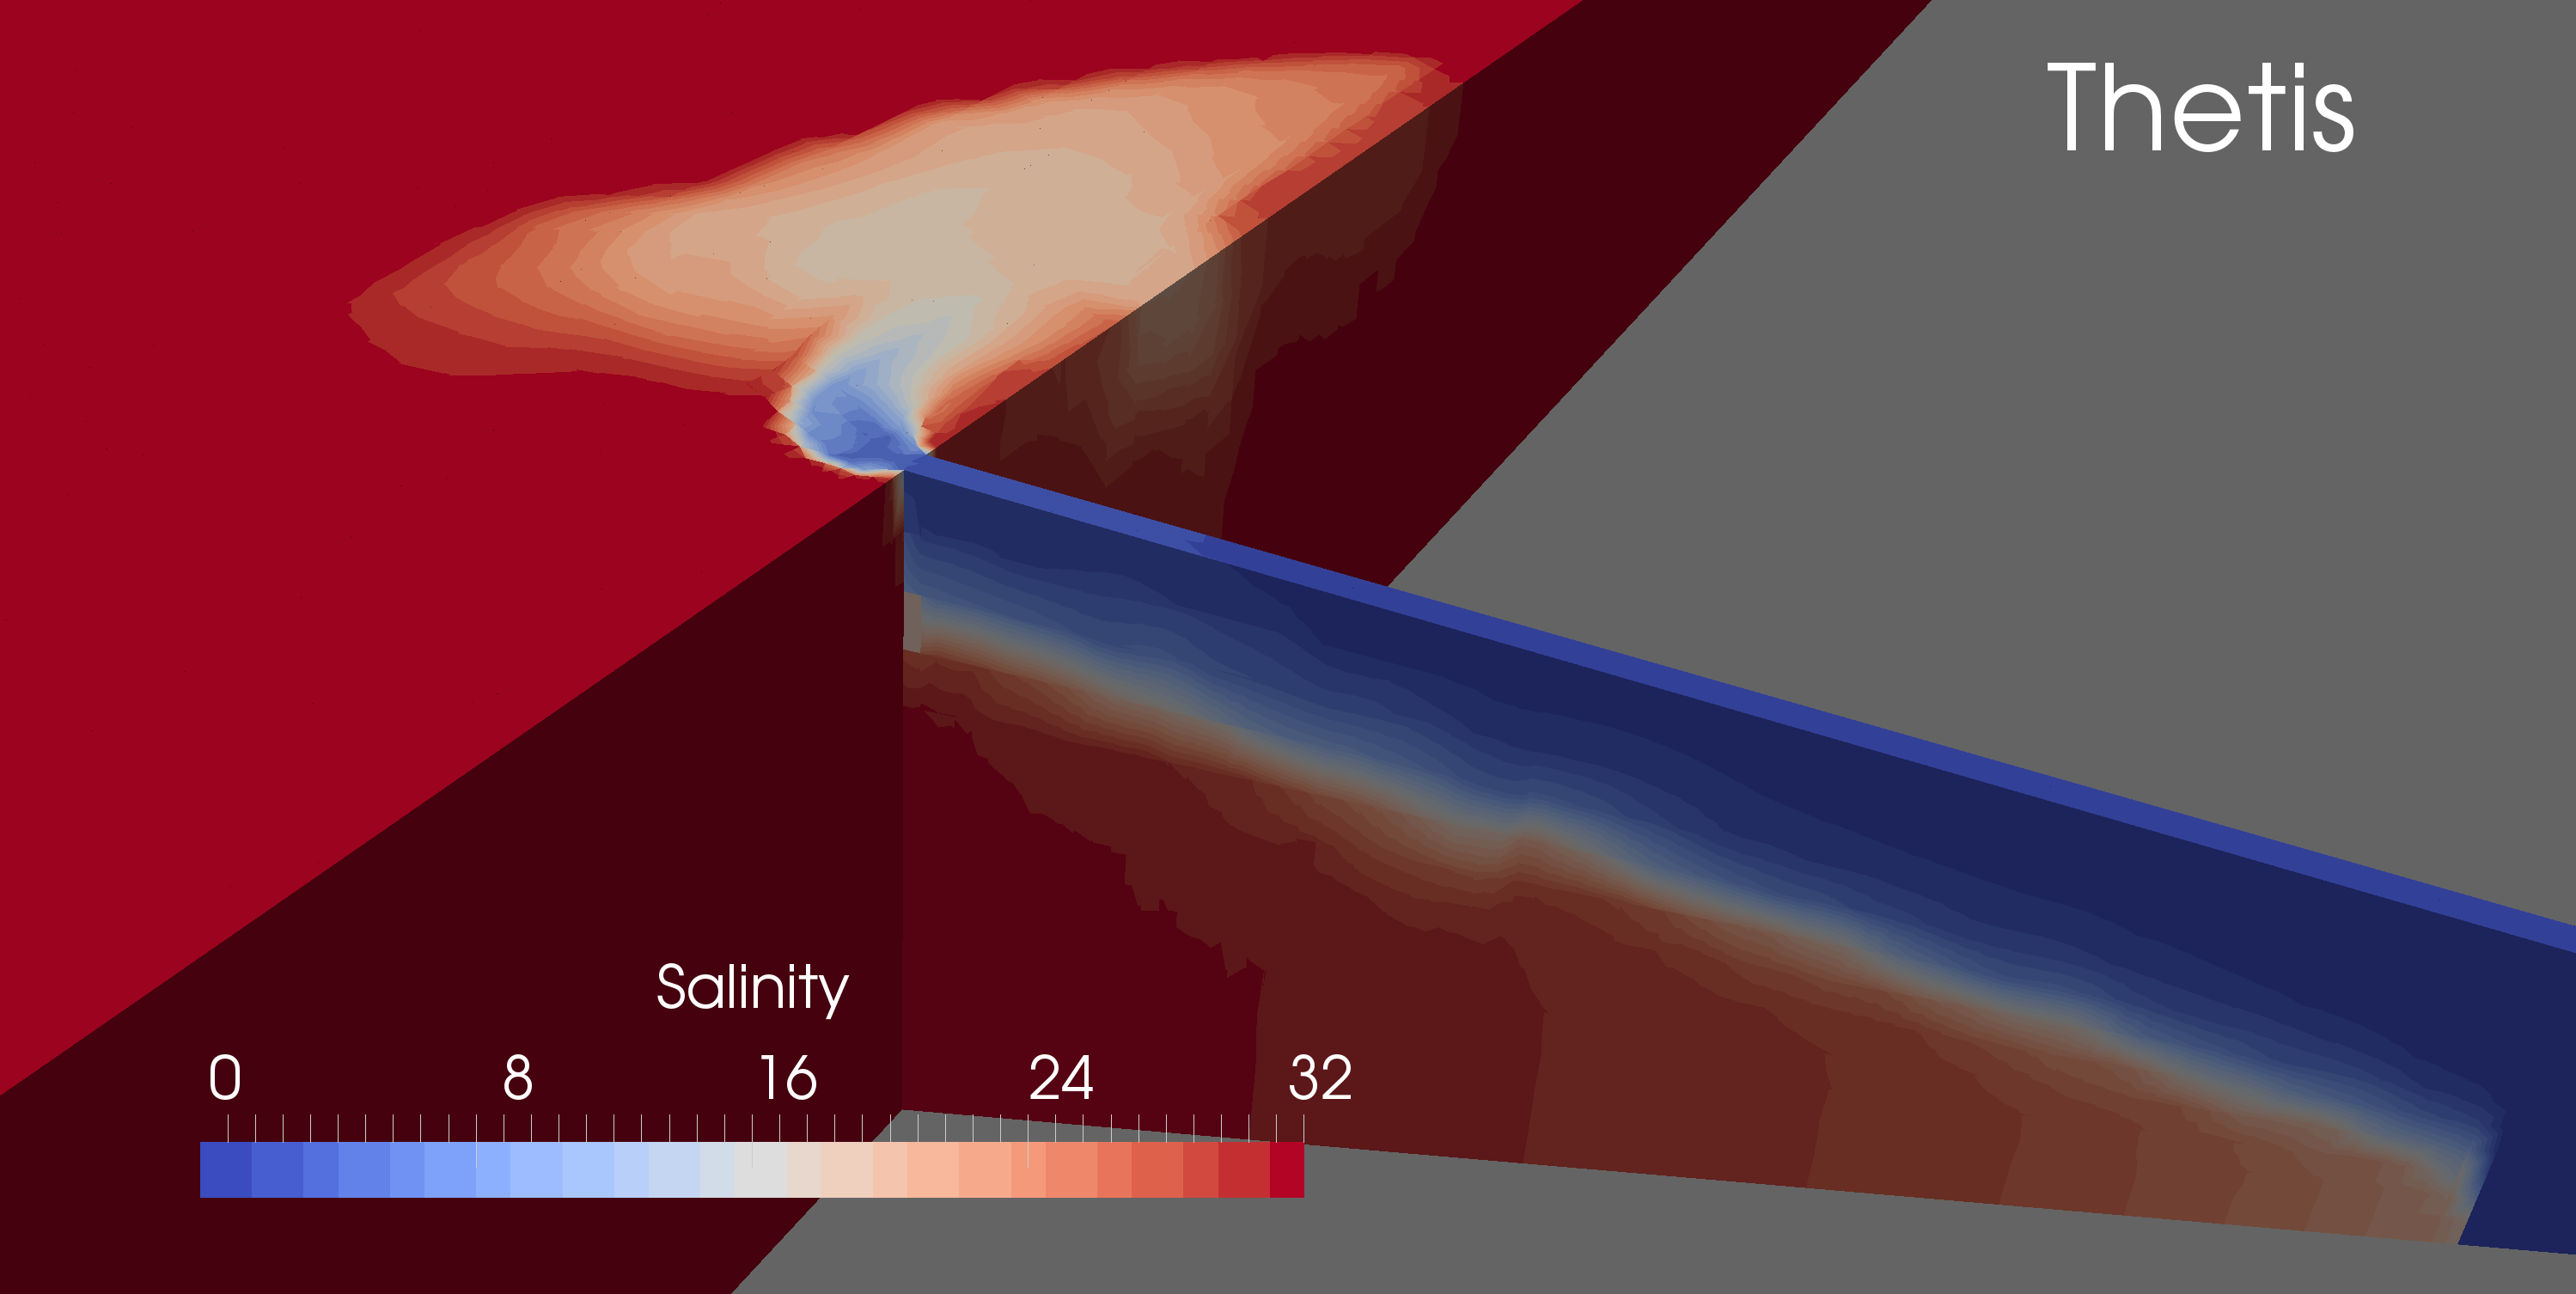
\includegraphics[width=0.8\textwidth]{thetis-rhine}\\
        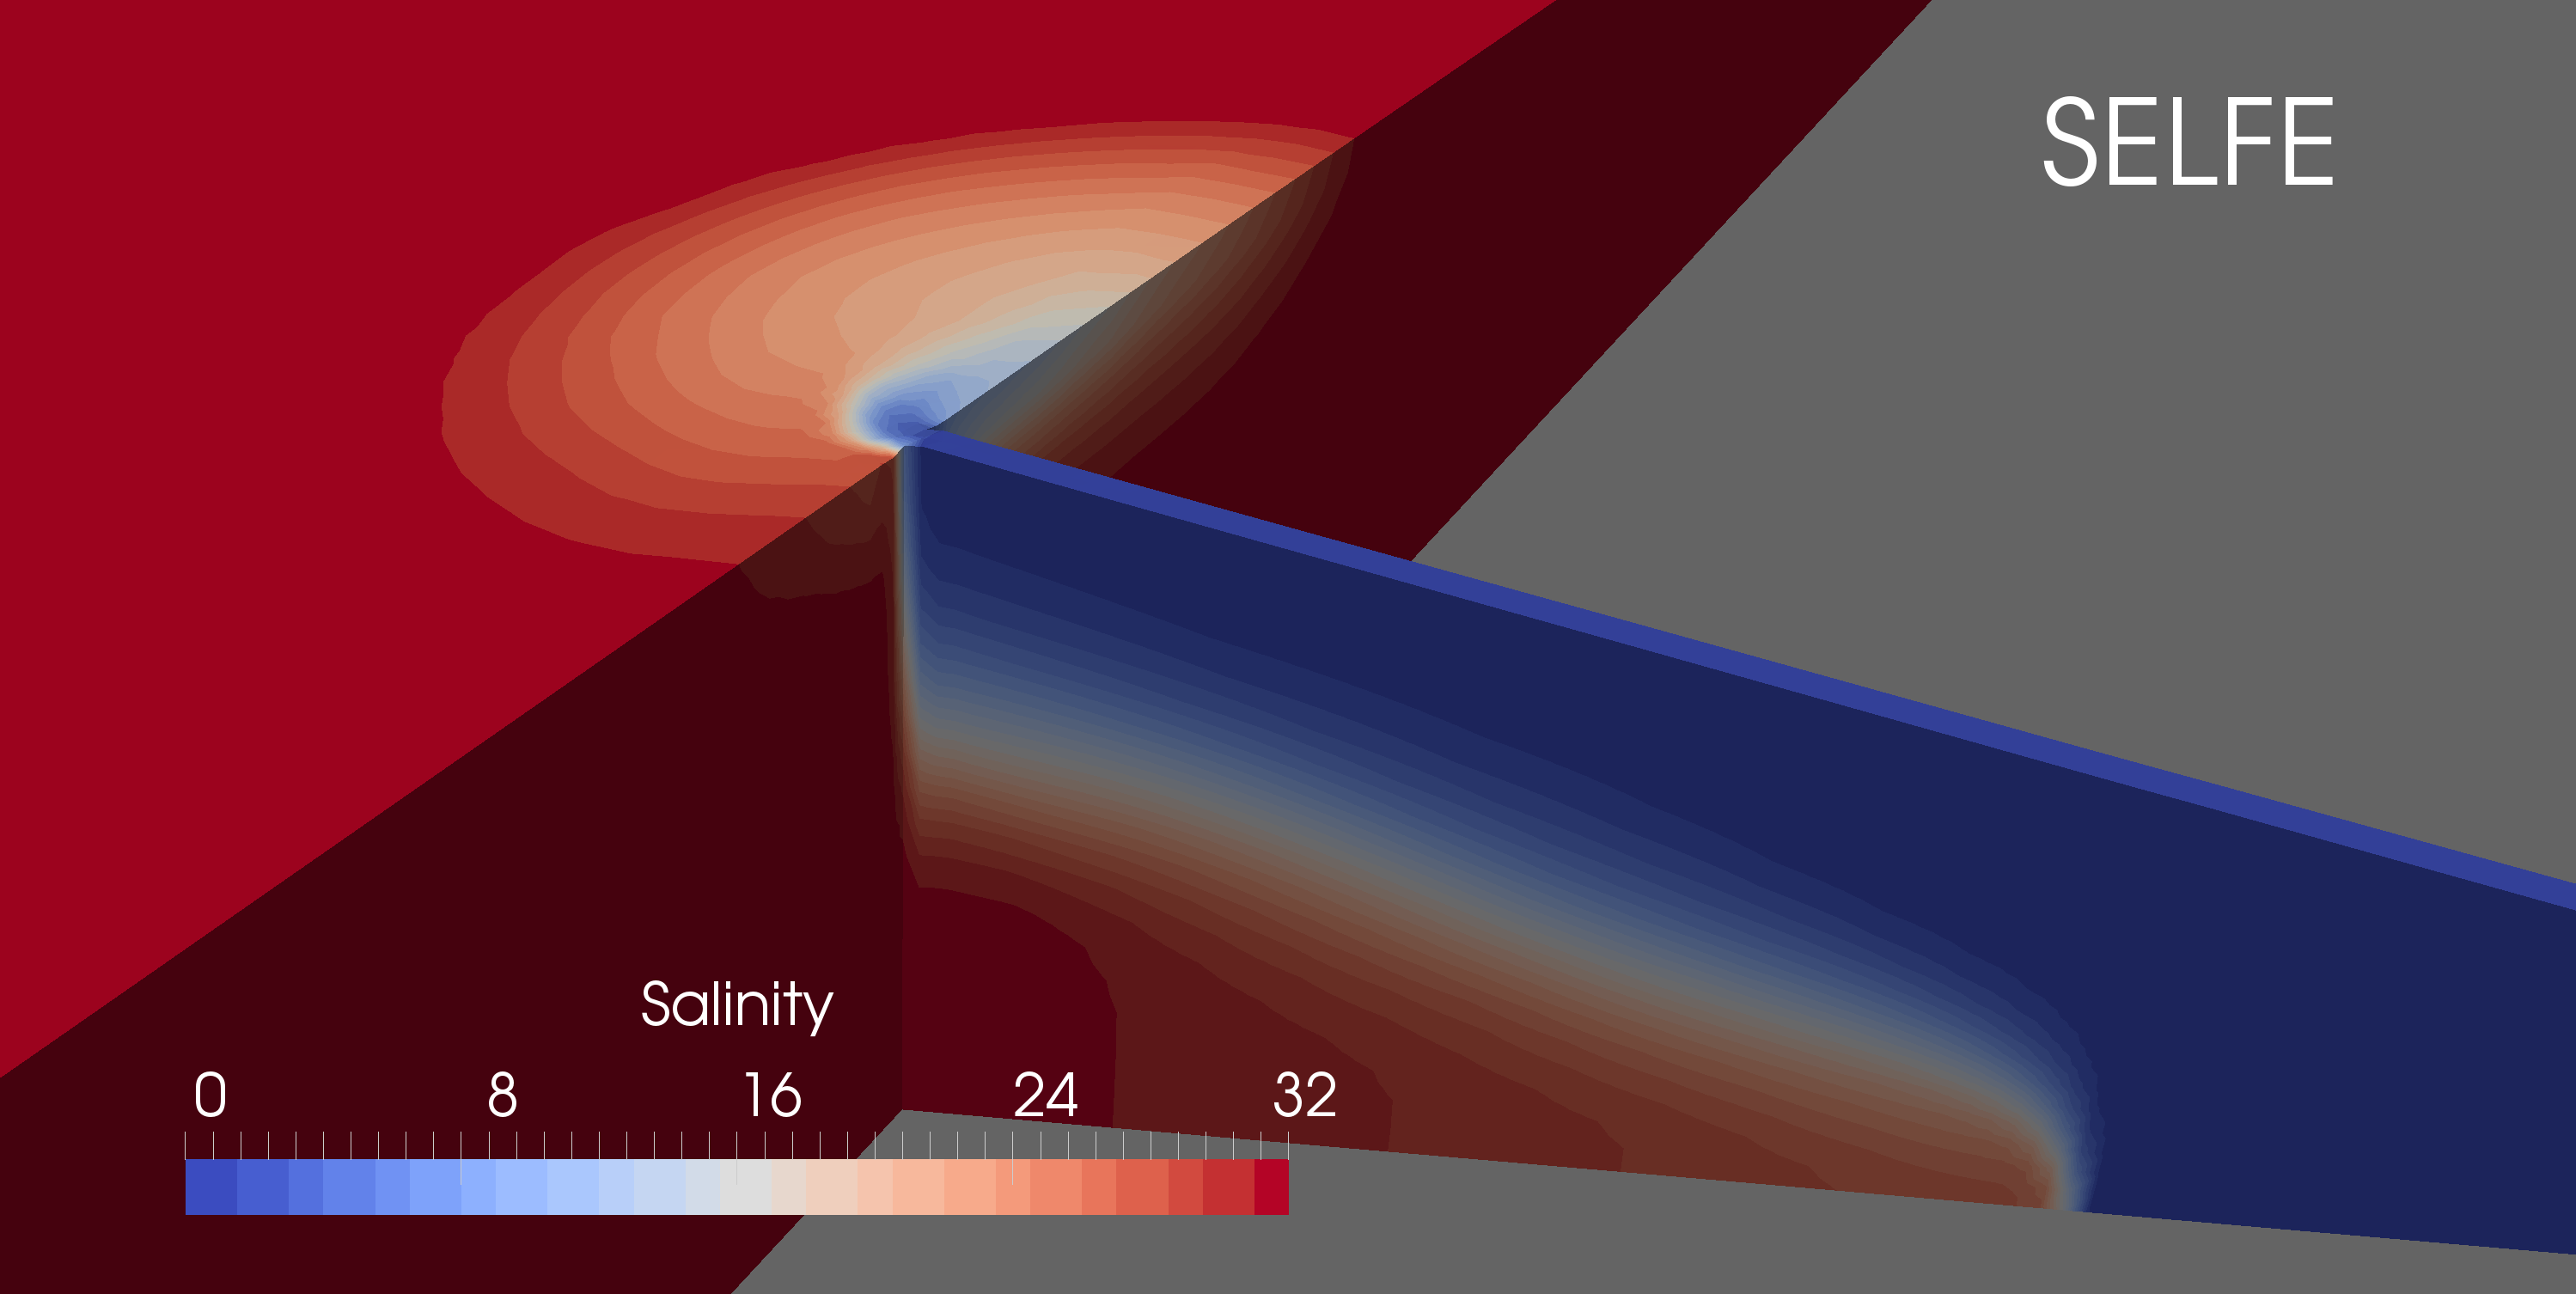
\includegraphics[width=0.8\textwidth]{selfe-rhine}
    \end{column}
    \hspace{-2em}
    \begin{column}{0.4\textwidth}
      Rhine ROFI test case from \cite{Boer:2006} \doilink{10.1007/s10236-005-0042-1}
    \end{column}
  \end{columns}
\end{frame}

\bgroup
\setbeamertemplate{background}{}
\begin{frame}[standout]
  \hspace*{-2em}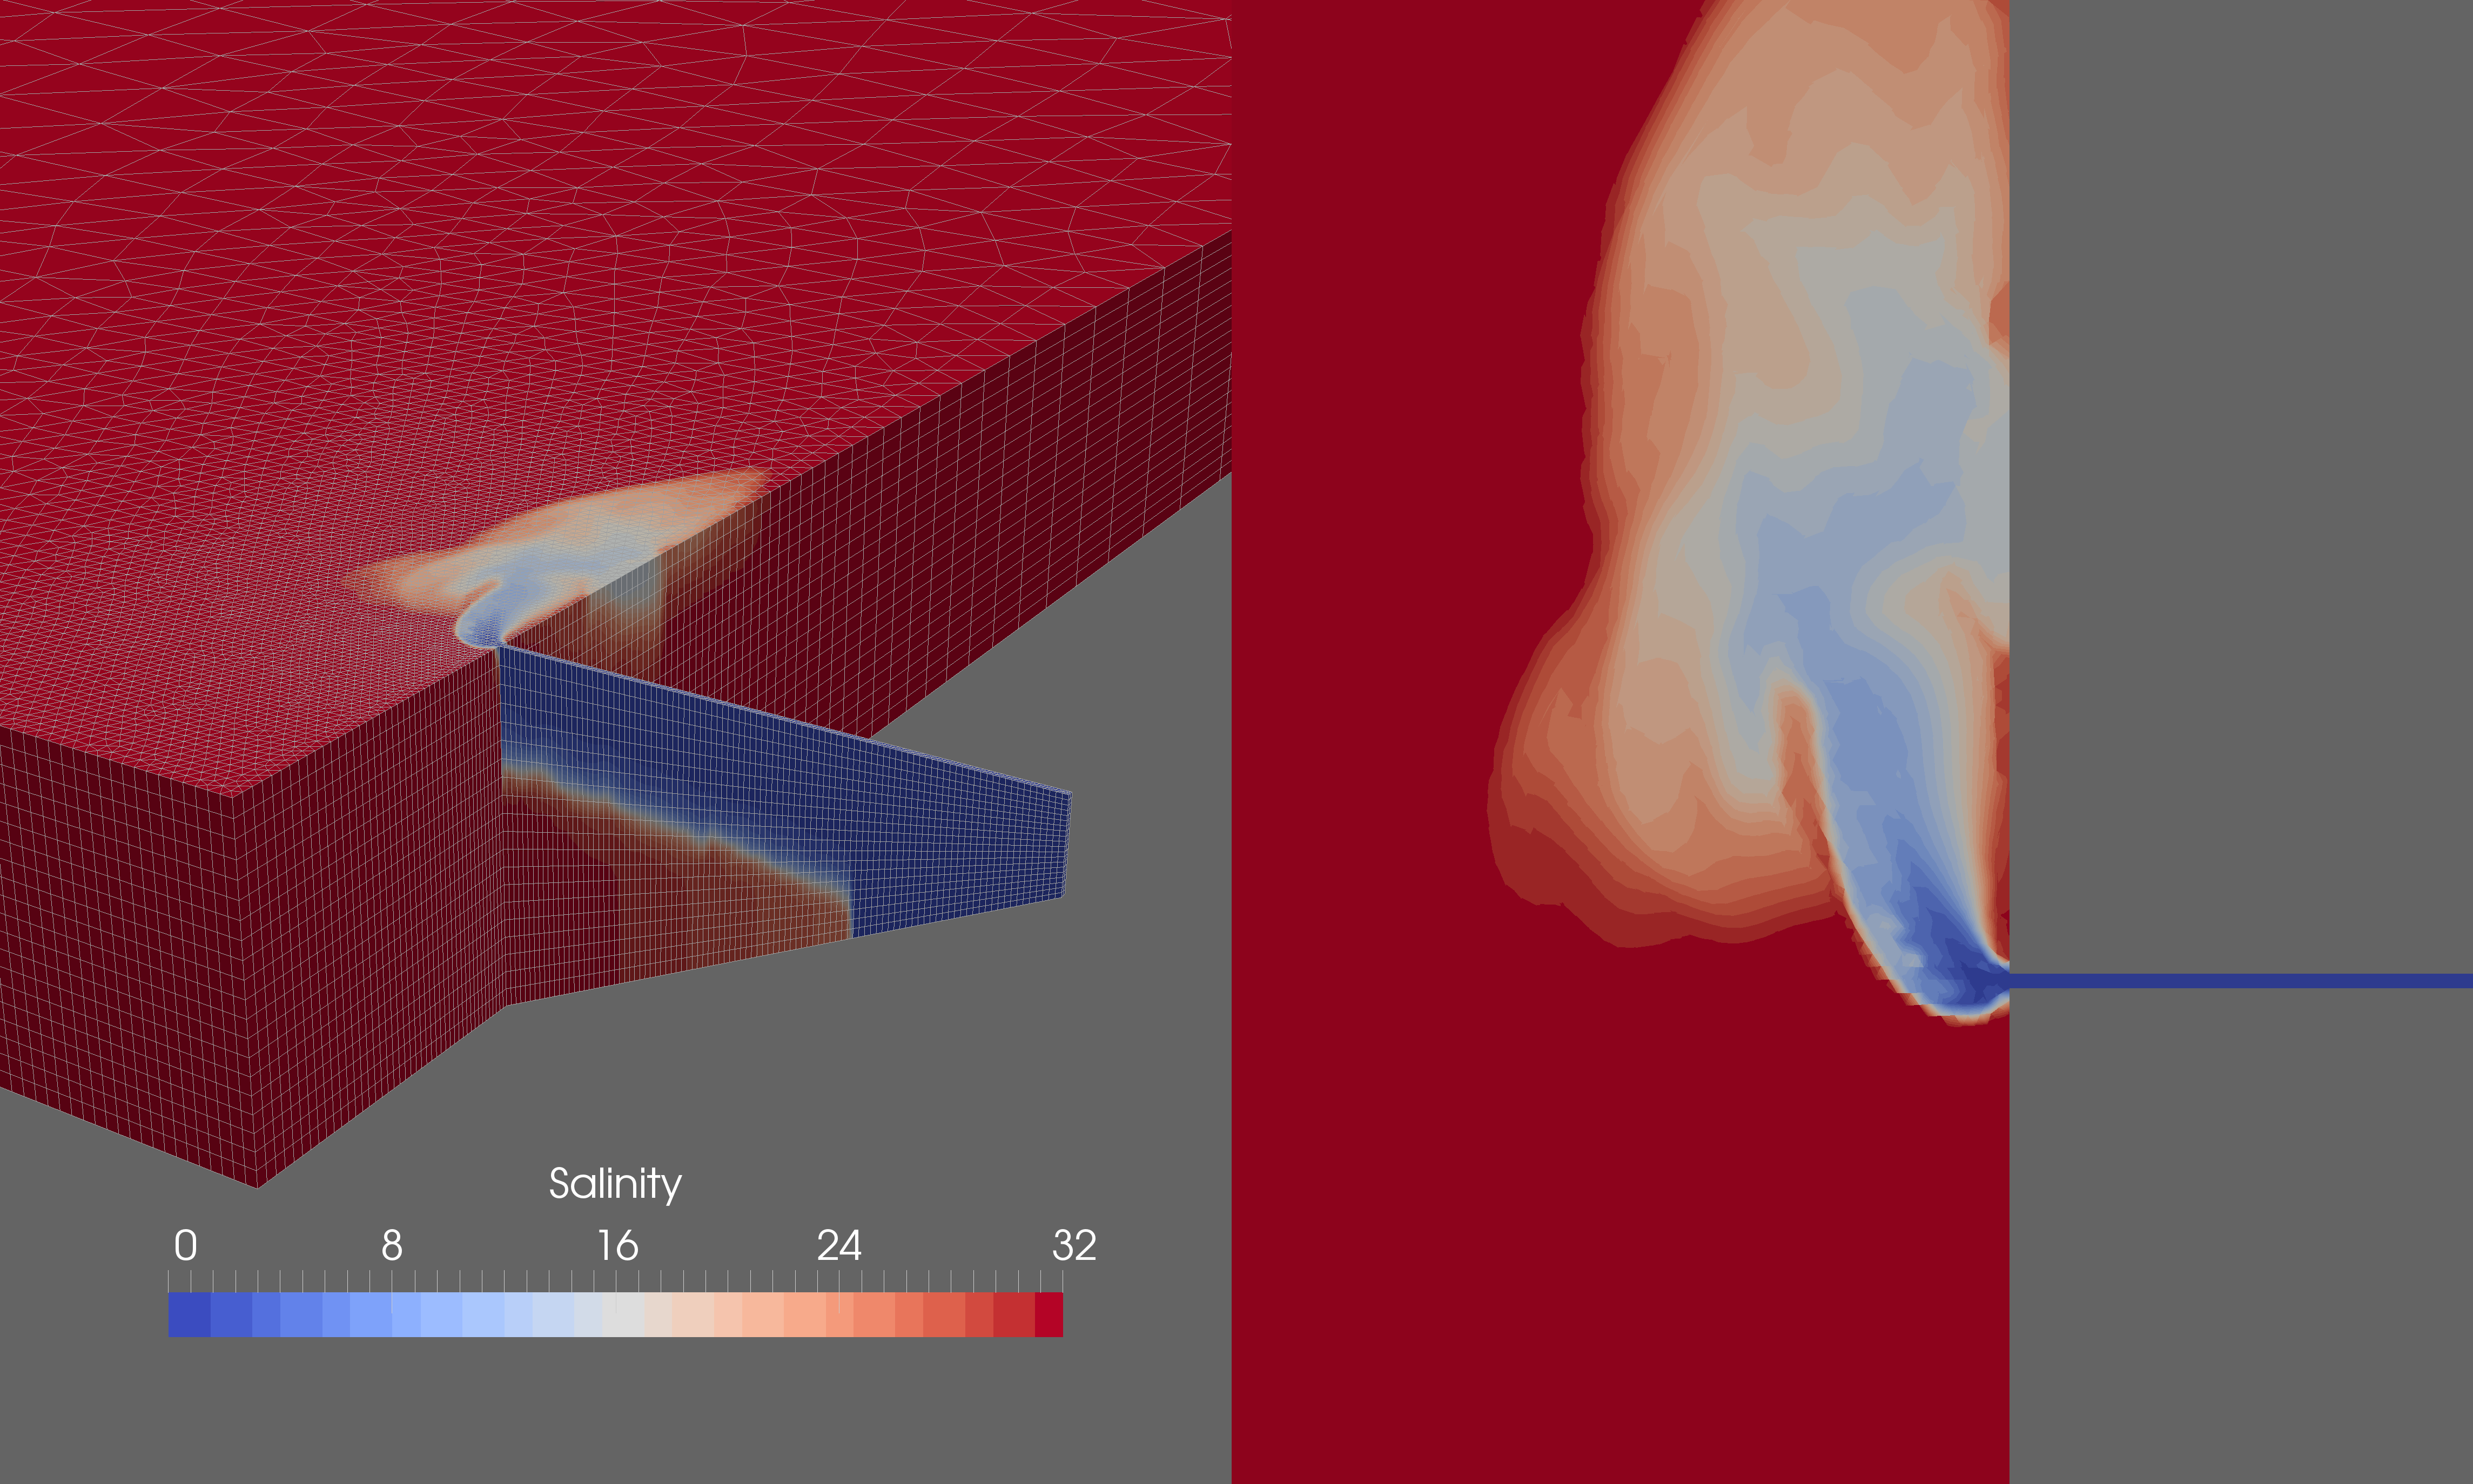
\includegraphics[width=\paperwidth]{thetis-rhine-hires}
\end{frame}
\egroup

\begin{frame}[fragile]
  \frametitle{Example configuration}
\begin{minted}[fontsize=\scriptsize]{python}
from thetis import *
mesh2d = Mesh(...)
V = FunctionSpace(mesh2d, "CG", 1)
bathymetry = Function(V, name="Bathymetry")
bathymetry.interpolate(...)
# Build timestepping solver
solver = solver.FlowSolver(mesh2d, bathymetry, nlayers)
options = solver.options
options.solve_salt = False
options.constant_salt = Constant(...)
options.solve_temp = True
# More options elided...
options.fields_to_export = ['uv_2d', ...]
# Create variational forms (also builds function spaces)
solver.create_equations()
init_temp = Function(solver.function_spaces.H, 
                     name="initial temperature")
init_temp.interpolate(...)
solver.assign_initial_conditions(temp=init_temp)
solver.iterate()
\end{minted}
\end{frame}

\begin{frame}[fragile]
  \frametitle{Time integrators}
  \begin{itemize}
  \item DIRK/ERK: just provide Butcher Tableau
\begin{minted}[fontsize=\scriptsize]{python}
class BackwardEuler(DIRKGeneric):
    a = [[1.0]]
    b = [1.0]
    c = [1.0]

class DIRK23(DIRKGeneric):
    "From DIRK(2,3,3) IMEX scheme in Ascher et al. (1997)"
    gamma = (3 + np.sqrt(3))/6
    a = [[gamma, 0],
         [1-2*gamma, gamma]]
    b = [0.5, 0.5]
    c = [gamma, 1-gamma]
\end{minted}
  \item IMEX: tag equations terms as explicit, implicit or source,
    will be treated appropriately
  \end{itemize}
\end{frame}
\section{Performance}

\begin{frame}[fragile]
  \frametitle{Programmer performance}
  \begin{onlyenv}<1>
    \begin{block}{Small code base}
\begin{minted}[fontsize=\scriptsize]{sh}
$ cloc thetis/
Language  files   blank   comment   code
Python       19    922      1726    5176
\end{minted}
      c.~1.5 person years
    \end{block}
  \end{onlyenv}
  \begin{onlyenv}<2->
    \begin{block}{Has an adjoint}
      \begin{onlyenv}<2>
\begin{minted}[fontsize=\scriptsize]{python}
# Import thetis
from thetis import *

mesh = PeriodicRectangleMesh(...)
V = FunctionSpace(mesh, "CG", 1)
bathymetry = Function(V, name="Bathymetry")
solver = solver.FlowSolver2d(mesh, bathymetry, order=1)
# Set up options
...
# Solve problem
solver.iterate()
\end{minted}
      \end{onlyenv}
      \begin{onlyenv}<3->
\begin{minted}[fontsize=\scriptsize,escapeinside=||]{python}
# Import thetis
|\colorbox{mLightBrown}{from thetis\_adjoint import *}|

mesh = PeriodicRectangleMesh(...)
V = FunctionSpace(mesh, "CG", 1)
bathymetry = Function(V, name="Bathymetry")
solver = solver.FlowSolver2d(mesh, bathymetry, order=1)
# Set up options
...
# Solve problem
solver.iterate()
\end{minted}
      \end{onlyenv}
    \end{block}
    \begin{visibleenv}<3->
\begin{minted}[fontsize=\scriptsize]{sh}
$ cloc thetis_adjoint/
Language  files   blank   comment   code
Python        1       0         0      4
\end{minted}
    \end{visibleenv}
  \end{onlyenv}
\end{frame}

\begin{frame}
  \frametitle{Computational performance}
  \begin{block}{\cite{Ilicak:2012} lock exchange test case}
    \begin{itemize}
    \item 512 triangles, 20 layers. 10k elements, 61k scalar dofs.
    \item 900s simulated time.
    \item Single core results.
    \end{itemize}
  \end{block}
{\small
  \begin{tabular}{lrr}
    Code ``version''               & Walltime & Simulated s/s \\
    \hline
    ``bendy'' FFC                  & c.~193s  & 4.7           \\
     TSFC (Feb.)                   & c.~145s  & 6.2           \\
    + COFFEE                       & c.~93s   & 9.7           \\
    + Tune solver/quadrature       & c.~64s   & 14            \\
    + PETSc fix                    & c.~37s   & 24            \\
    + SSPRK3$\rightarrow$ERK2-LPUM & c.~19s   & 47            \\
  \end{tabular}

\only<2>{SLIM $P_1dg-P_1dg$ model requires c.~148s (6.1x)}
\only<3>{Fluidity $P_1dg-P2$, non-hydrostatic, tets c.~1000s (0.9x)}
}
\end{frame}

\begin{frame}
  \frametitle{And finally}
  \begin{itemize}
  \item More rigorous performance benchmarking
  \item Better solvers (especially for mimetic case)
  \item Validation
  \item ...
  \end{itemize}

  \begin{block}{Acknowledgments}
    \begin{center}
      \raisebox{5pt}{
\includegraphics[width=0.4\textwidth]{nerc-logo}}
      \hfil\raisebox{0pt}{
\includegraphics[width=0.3\textwidth]{epsrc-logo}}
    \end{center}
    \begin{center}
      \raisebox{0pt}{
\includegraphics[width=0.15\textwidth]{nsf-logo}}
      \hfil\raisebox{5pt}{
\includegraphics[width=0.3\textwidth]{xsede-logo}}
      \hfil\raisebox{15pt}{
\includegraphics[width=0.25\textwidth]{tacc-logo}}
    \end{center}
  \end{block}
\end{frame}
\appendix
\begin{frame}[t]
  \frametitle{References}
  \printbibliography[heading=none]
\end{frame}


\end{document}
